

\section{Results and Analysis}

\subsection{Dirichlet Process Clustering}
The result of our clustering is presented in Fig \ref{clustering_results}.
We can see that the method managed to accurately group up the data from the same environment with only one miss classified episode in arc-based representation.
Further investigation shows this is a rather small episode containing only 9 interaction data. 
It is likely that when expressed in arc-based representation, the data in this episode happen to exhibit similar outcomes in both environments which finally led to this confusion.
However, another feature of the clustering result is that data from the same environment can spread in multiple clusters, and we even have many clusters containing only one episode.
There are two possible reasons for this phenomenon.
One is that some execution is very noisy, hence if an episode happens to include such interaction data, it might appear to be largely different from the rest of the episodes.
Another possible reason is that we applied posterior convergence too soon, and the weights calculated using Eq. (\ref{refitted_weights}) over-fits to the existing data, hence preventing further data from joining the cluster.
Fortunately, this should not affect the model prediction too much.


\begin{figure}[h]
\centering
\subfloat[]{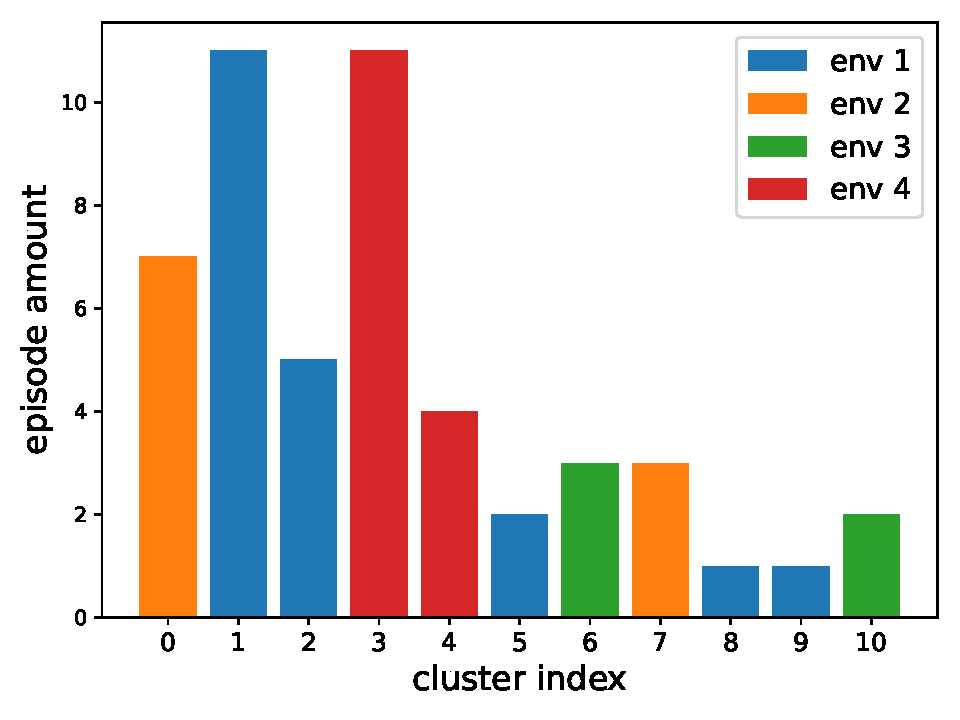
\includegraphics[width=0.22\textwidth]{xy_cluster_data.pdf}
%\label{a}
}
%\hfil
\subfloat[]{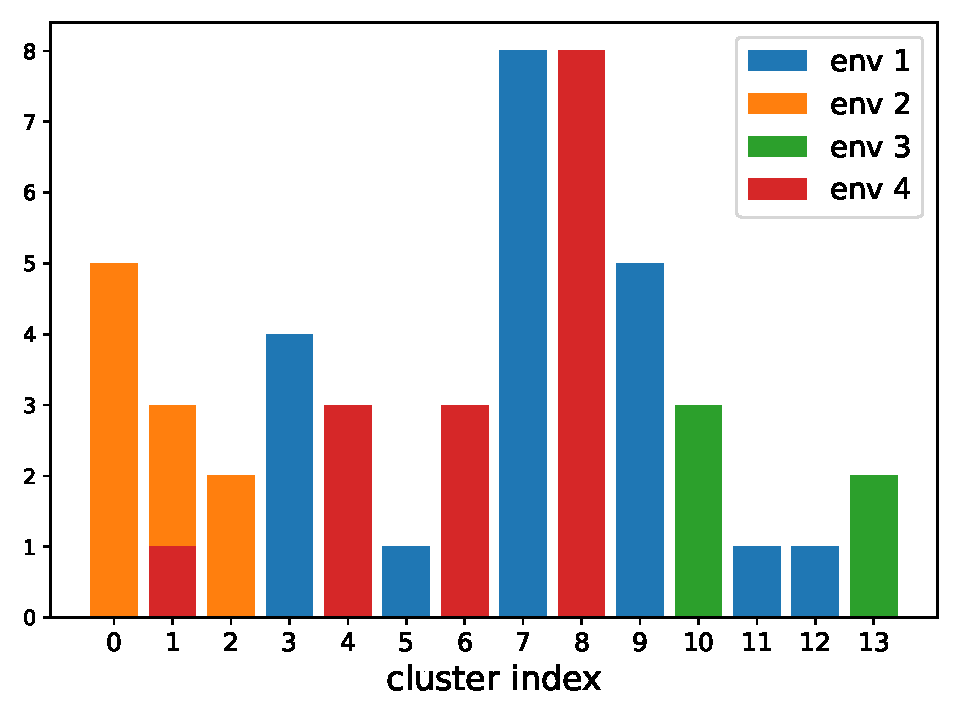
\includegraphics[width=0.22\textwidth]{arc_cluster_data.pdf}
%\label{b}
}
\caption{Cluster assignment of the data in Table \ref{data} after applying our DP clustering method.
(a) is the result using displacement-based representation, and (b) is the one for arc-based representation.}
\label{clustering_results}
\end{figure}


\begin{figure*}[!t]
\centering
\subfloat[]{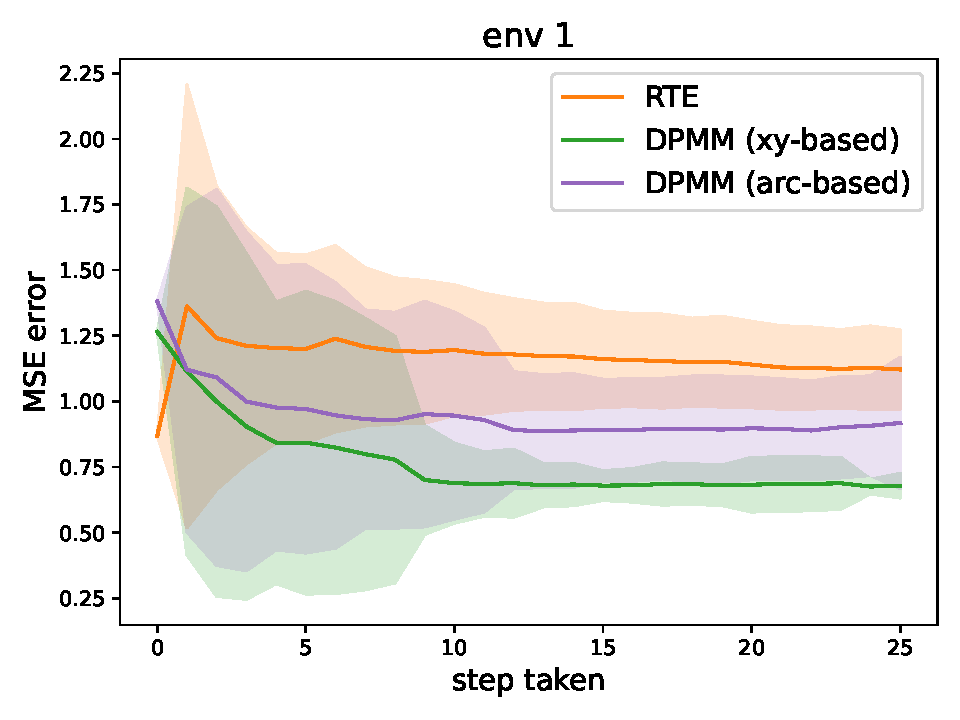
\includegraphics[width=0.45\textwidth]{regular_case0.pdf}%
\label{case_0}}
%\hfil
\subfloat[]{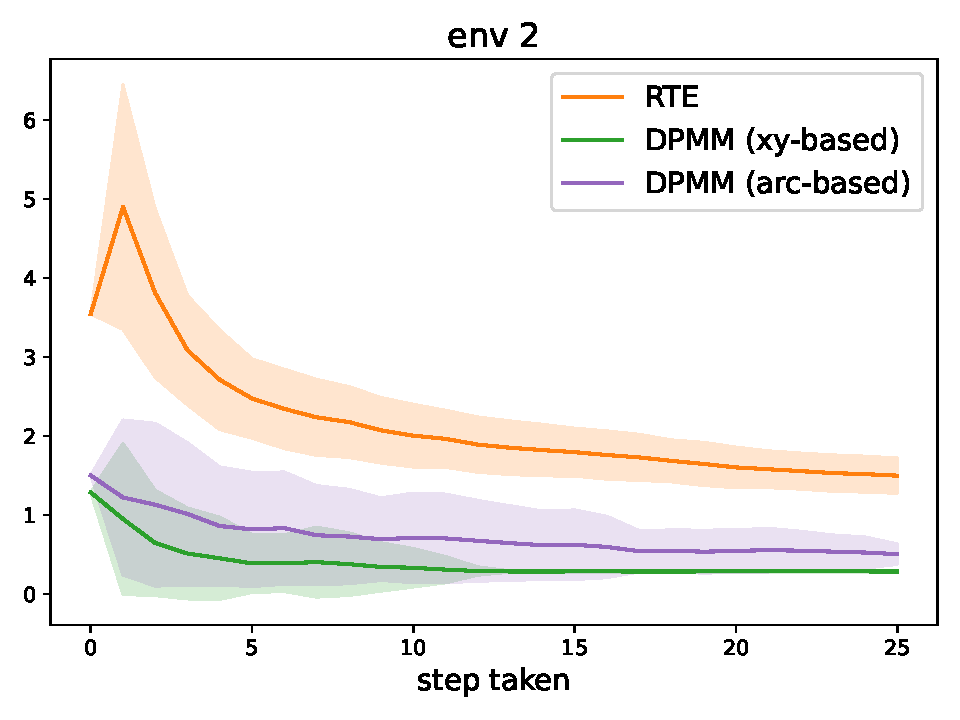
\includegraphics[width=0.45\textwidth]{regular_case1.pdf}%
\label{case_1}}
\vfil
\subfloat[]{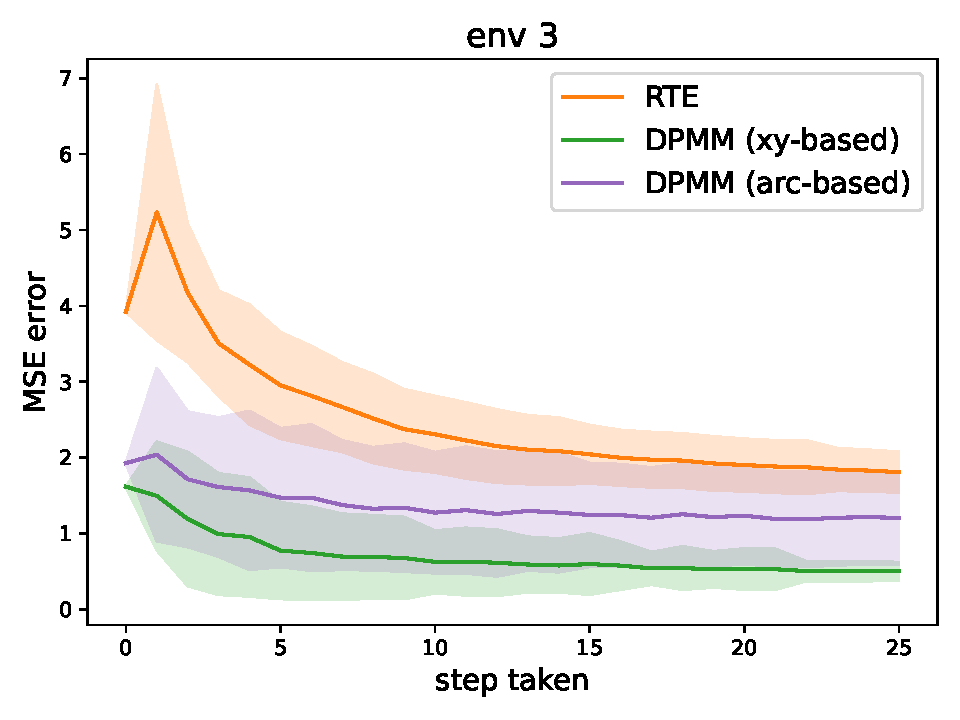
\includegraphics[width=0.45\textwidth]{regular_case2.pdf}%
\label{case_2}}
%\hfil
\subfloat[]{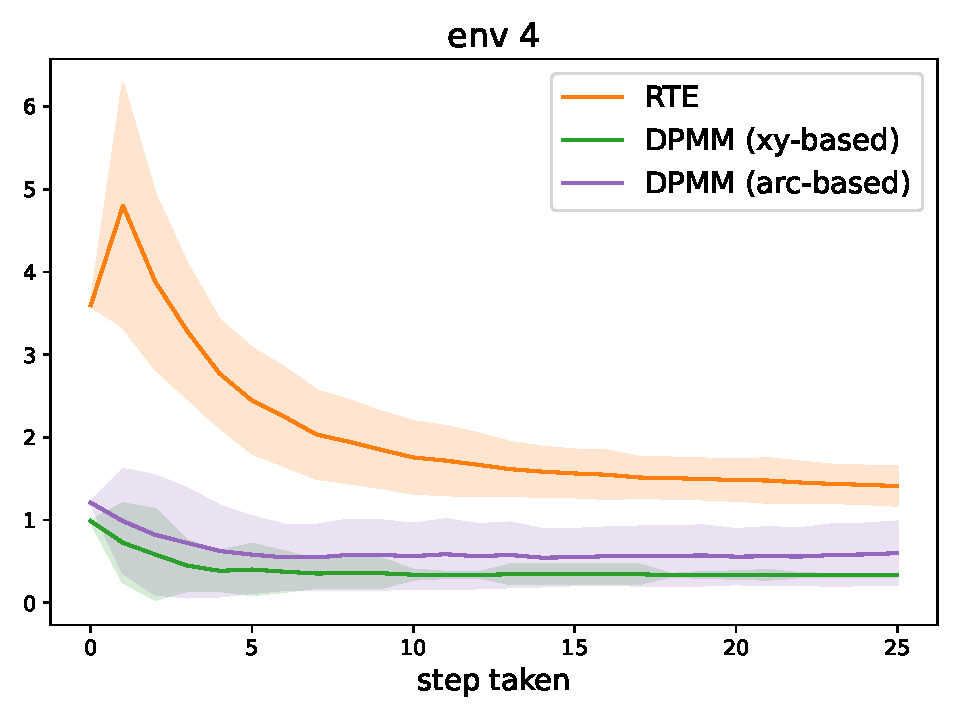
\includegraphics[width=0.45\textwidth]{regular_case3.pdf}%
\label{case_3}}
\caption{The prediction error versus the step taken in each environment.
The error is defined to be the mean-squared distance between the predicted final position and the actual final position.
}
\label{dynamics_learning}
\end{figure*}

\subsection{Dynamics Learning}
Before deploying the robot in the maze, we first test the capability of our robot to quickly learn the dynamics using the infinite mixture of GP model.
We do this by placing our robot in a previously encountered environment and feeding the robot with a randomly selected interaction data in each step.
We then make the robot predict the outcomes for the entire repertoire and monitor the change of the prediction error.
This is to simulate the model-based online adaptation process where the robot executes a policy in each time-step and use the outcome to update its model.
To mitigate the randomness in the result, we repeat this 100 times and plotted out the mean and standard deviation in Fig \ref{dynamics_learning}.


We can see that for any previously encountered environment, our model greatly outperforms the RTE method.
Surprisingly, the displacement-based method is significantly better than the arc-based method.
The displacement-based method can typically reduce the error to below $1.0$ within 5 steps, while the arc-based method learns much slower and is lesser stable.
This could result from the fact that arc-based method uses three parameters unlike the use of two parameters in displacement-based representation.
It's likely that the extra dimension and the inconsistent measurement error in arc-based method induces more uncertainties than displacement-based approach and also make the selection of the prior lesser stable.
Nevertheless, both infinite mixture of GP methods are much better than RTE.
This suggests that it is a successful method to prepare candidate priors from the historical data and try to figure out the most suitable one with the data collected online.
We also see that the RTE starts up with a increase in error.
This is likely a sign that the use of $x$ and $y$ displacements as the input space fails to handle the case where two policies leading to similar displacements in the default simulation environment create distinct outcomes in a new environment.
This explains the rapid increase in the error as such input space could generate misleading result.
It is counter-intuitive to see that env 1 has the largest error while it is most similar to the default environment.
Further investigation finds it hard to achieve an error lesser than 0.6 in env 1.
It is also found that environments closer to the default one have larger uncertainties in policy execution.
This is likely because the effect of random perturbation will accumulate during the motion, and the faster the robot walks the greater the uncertainties will be.
The data size collected from each environment matters as the learning in env 4 (15 episodes) is the fastest, while that in env 3 (5 episodes) is slowest.

\begin{figure*}[!t]
\centering
\subfloat[]{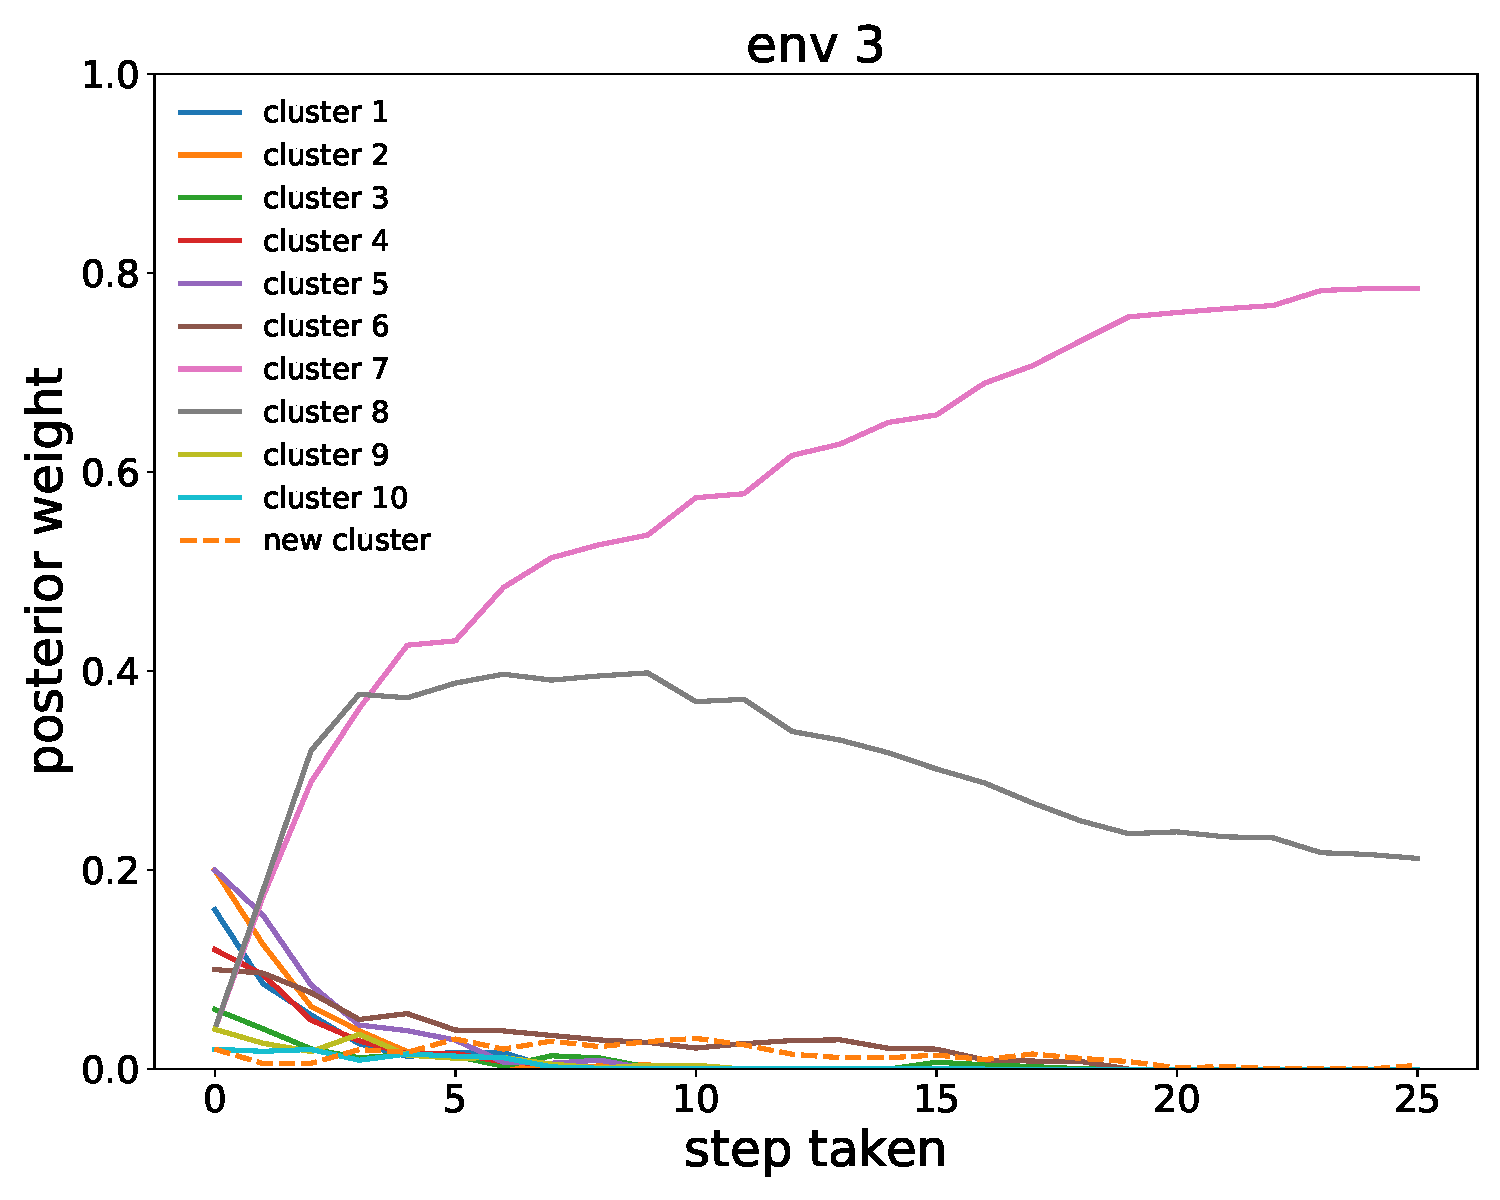
\includegraphics[width=0.45\textwidth]{weight_2.pdf}%
\label{weight_2}}
%\hfil
\subfloat[]{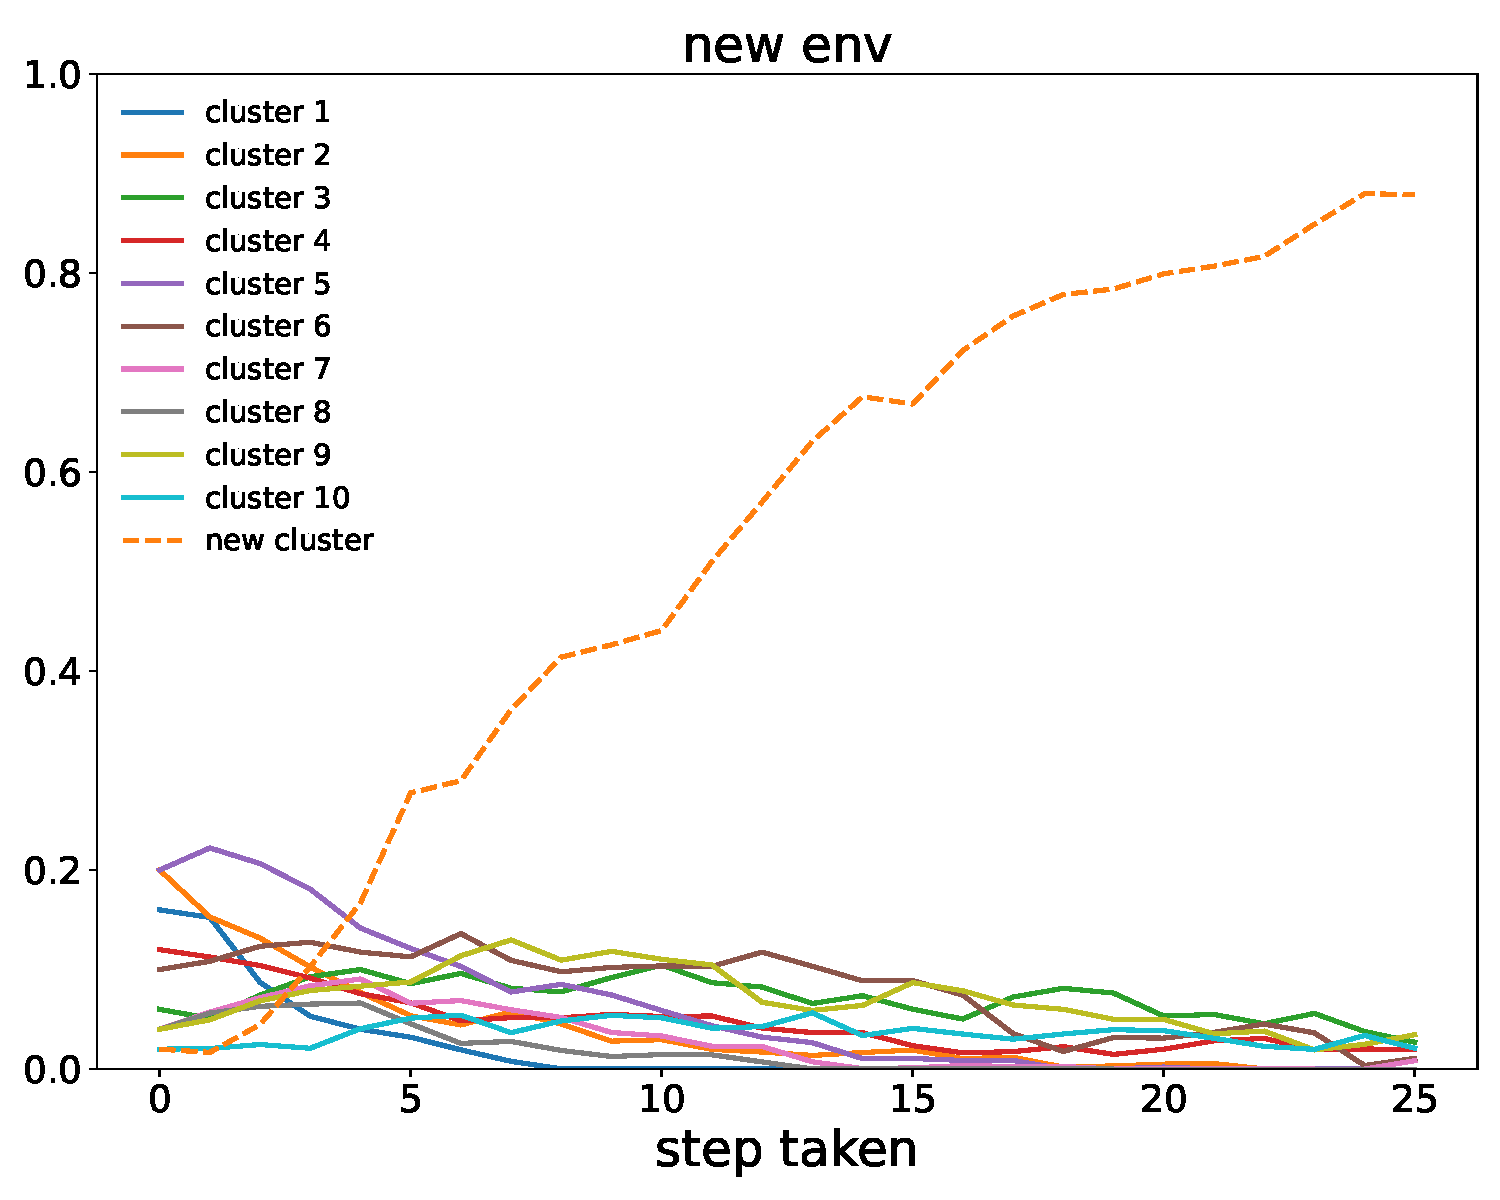
\includegraphics[width=0.45\textwidth]{weight_4.pdf}%
\label{weight_4}}
\caption{The change of the posterior weight of each cluster versus the number of steps taken.
These data correspond to the model using displacement-based dynamics representation.
}
\label{weights}
\end{figure*}

\begin{figure}[h]
\centering
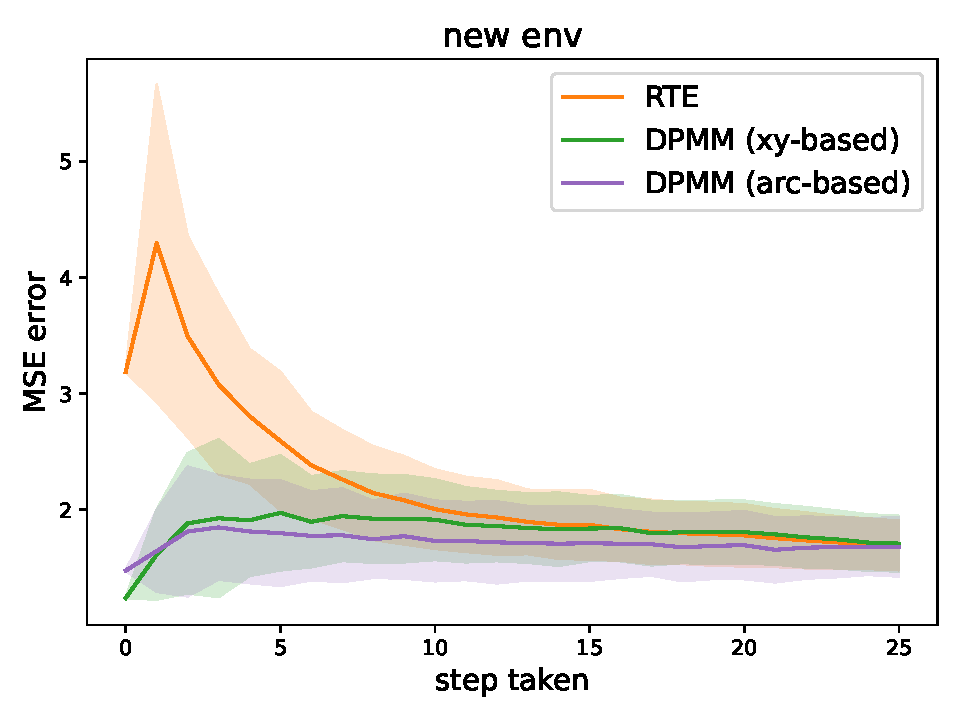
\includegraphics[width=0.45\textwidth]{regular_case4.pdf}
\caption{Dynamics learning in an unseen environment.
For this environment, the robot damage is in the leg 4, the friction coefficient is 0.77 and the torque scale is 0.82}
\label{new_env}
\end{figure}

These online learnings are all made in previously encounter environments.
To examine the generalizability of our method, we also tested the adaptation on a new environment.
It can be seen from Fig \ref{new_env} that although this environment is new hence none of the historical data will help, our method still manges to adapt in this environment as good as RTE.
To monitor the selection of the prior during the adaptation, we plotted out the posterior weights of each cluster, namely the $p(c=j| \bm{x}_{1:N})$ in Eq. (\ref{predicted_mean}).
We see from Fig \ref{weight_2} that although the data for env 3 split into two clusters (see Fig \ref{clustering_results}), they collectively contribute to most of the posterior weights.
When deployed in the new environment, none of the existing clusters can explain the interaction data.
Thanks to the wonderful property of DP that the probability for getting a new cluster is never zero, we see from the posterior weights in Fig \ref{weight_4} that the robot eventually realizes that it is in a new situation and hence uses RTE to make prediction.


Finally, we tested our model's capability of learning new dynamics.
This is done by adding an episode of new data to our dataset and updating our model accordingly.
This episode is collected from the new environment in Fig \ref{new_env} and contains 35 data.
The result is presented in Fig \ref{new_adapt}.
We see that after incorporating this new episode into our dataset, the robot using displacement-based method quickly learns how to adapt in this new environment.
The arc-based method is also performing better, but it learns slower.

\begin{figure}[h]
\centering
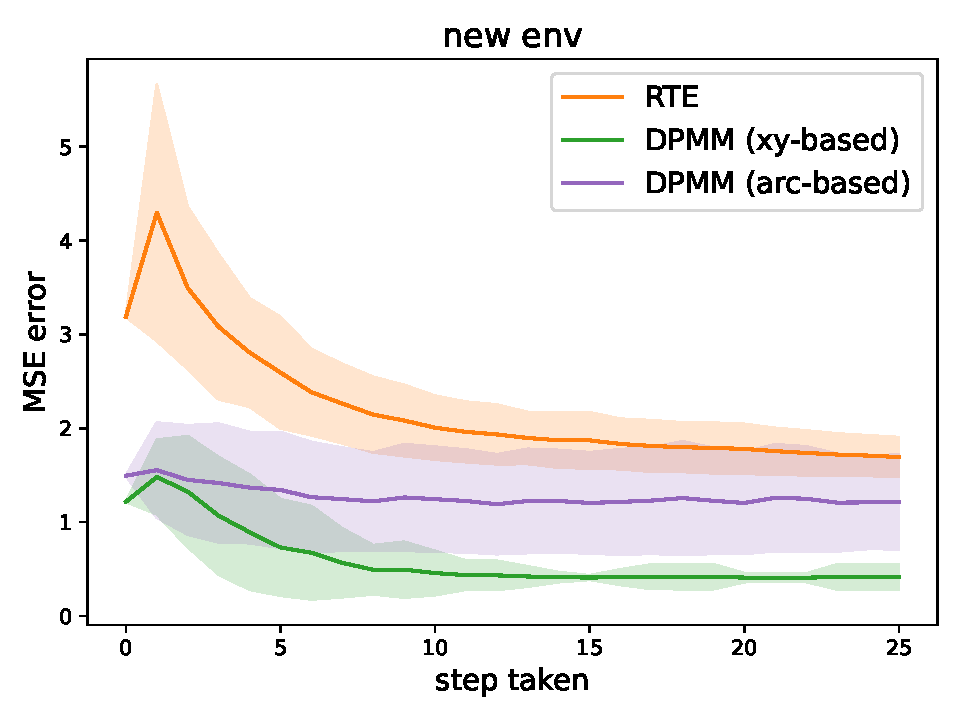
\includegraphics[width=0.45\textwidth]{new_case4.pdf}
\caption{Dynamics learning performance after having collected an episode of interactions from this environment.
With dataset updated, 20 extra Gibbs sampling sweeps were conducted to identify the best indicator configuration.}
\label{new_adapt}
\end{figure}


\begin{figure*}[!t]
\centering
\subfloat[]{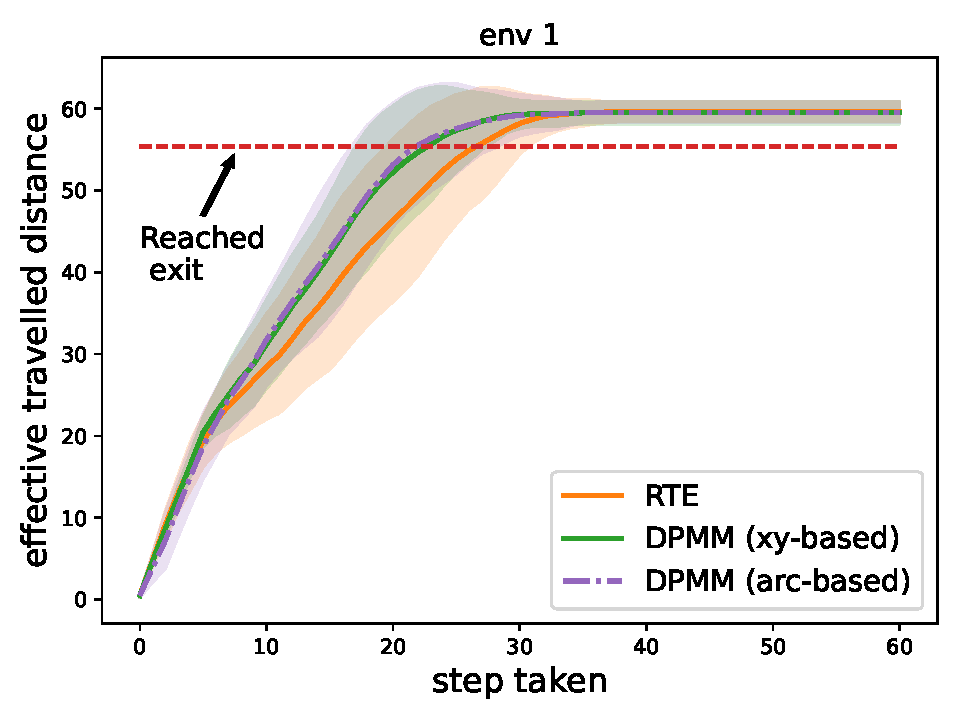
\includegraphics[width=0.45\textwidth]{navigation_results_0.pdf}%
\label{maze_0}}
%\hfil
\subfloat[]{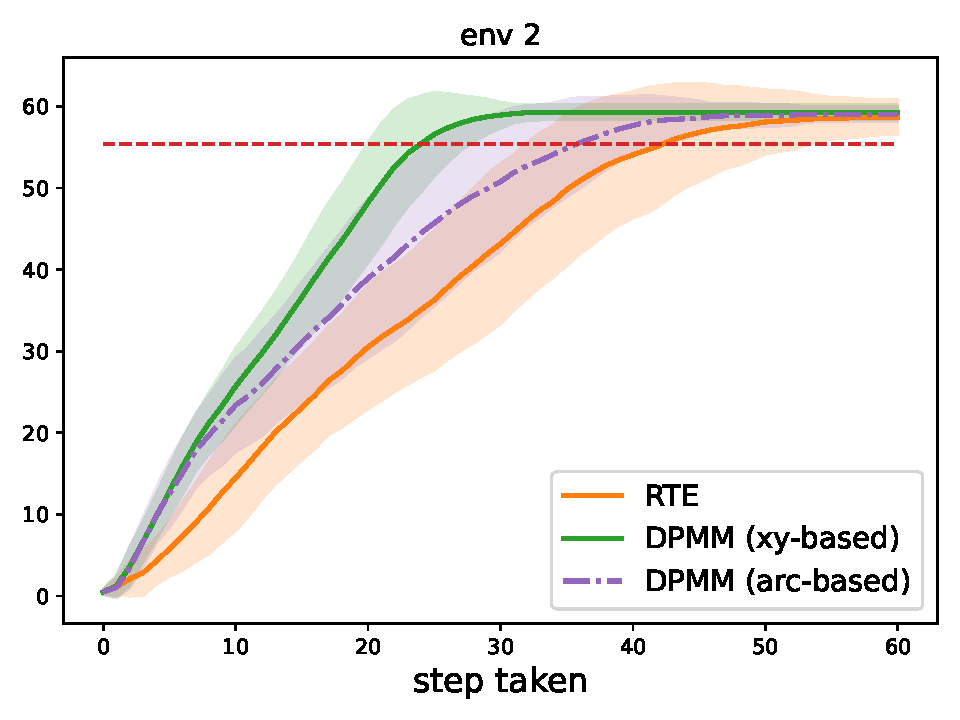
\includegraphics[width=0.45\textwidth]{navigation_results_1.pdf}%
\label{maze_1}}
\vfil
\subfloat[]{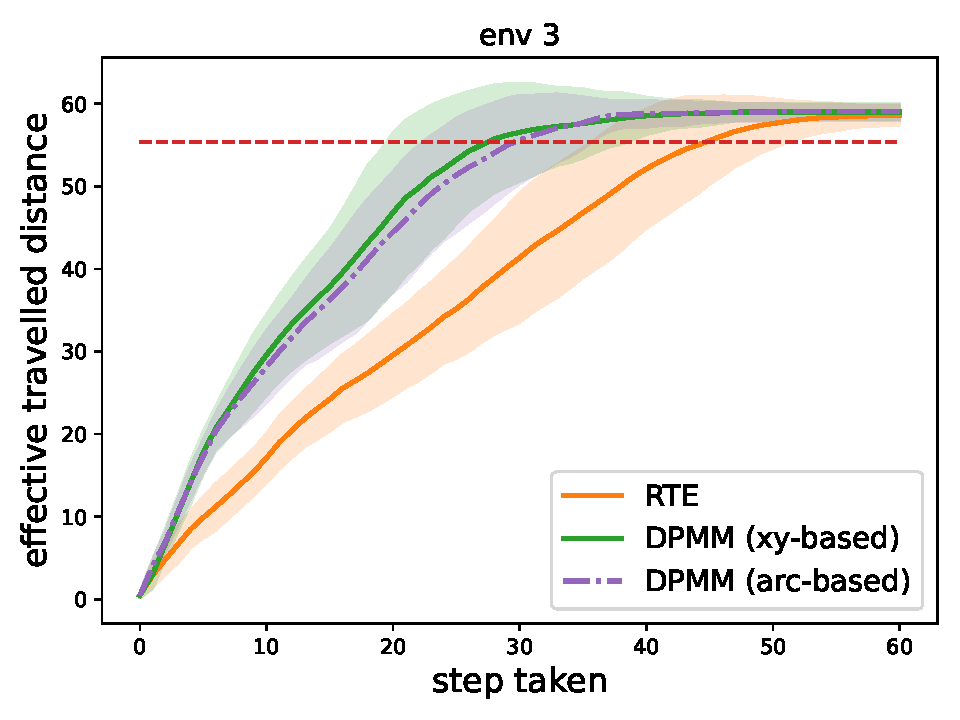
\includegraphics[width=0.45\textwidth]{navigation_results_2.pdf}%
\label{maze_2}}
%\hfil
\subfloat[]{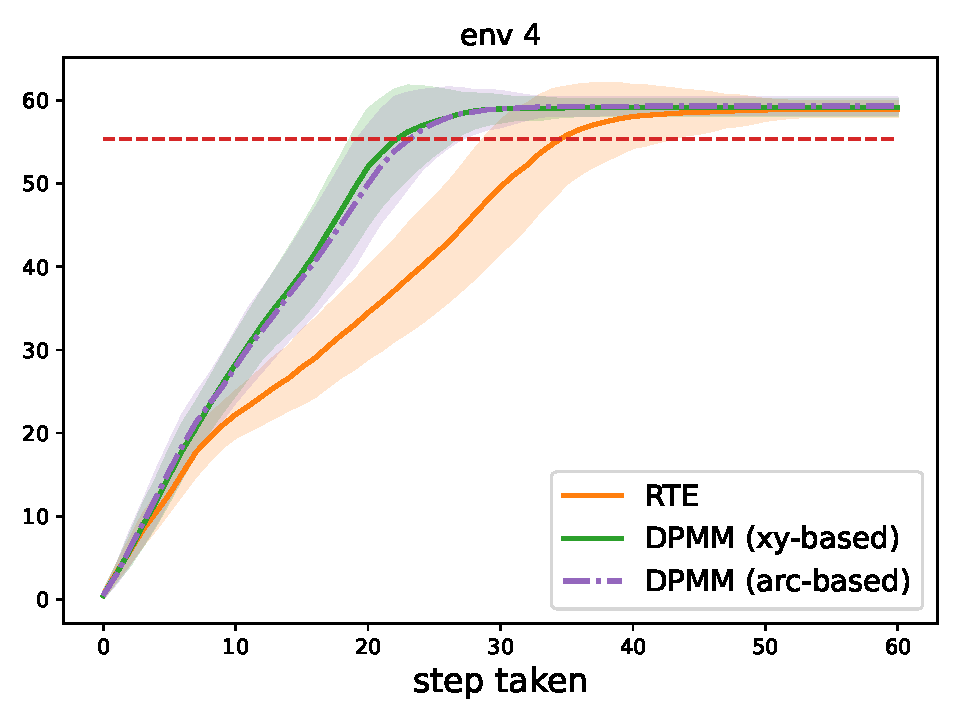
\includegraphics[width=0.45\textwidth]{navigation_results_3.pdf}%
\label{maze_3}}
\caption{The maze adaptation performance of the robots using different models.
To avoid getting any unrepresentative results due to initial state, we randomly initialize the robot 100 times.
Each time the robot is randomly placed in the starting area with orientation $\theta \sim \mathcal{N}(0, 30^{\circ})$.
Since the maze is U-shaped, we use effective distance instead of the distance to the goal to track the progress of the robot.
The effective distance is defined to be the projection on the suggested path, which is the distance on the path that is closet to the robot's current position.
The effective distance at the exit is 55.386.
}
\label{navigation_results}
\end{figure*}


\subsection{Maze Adaptation}


Since our method shows very promising result in dynamics learning, we hoped to
investigate the practical significance of this improvement in actual task solving.
We deployed our robot in each of the previously encountered environments and let it navigate through the maze.
The results are presented in Fig \ref{navigation_results}. 
We see that in all environments, the robots using our models completes the task significant faster than the one using RTE.
Although we have found that the displacement-based method provides much more accurate modelling of the dynamics than the arc-based method, the two robots showed little difference in performance except in env 2.
A very likely explanation for this is that for the policies that are used most often, the two methods provide similar accuracies.
By examining the plots, we see that most curves experience a decrease in its gradient at effective distance roughly equals to 20.
Referring to the floor-plan of the maze in Fig \ref{maze}, this effective distance corresponds to the first turning, after which the tunnel width is halved.
This poses a tougher requirement of the model predictions, which may otherwise lead to collisions.
We can see from Fig \ref{maze_0} and Fig \ref{maze_3} that the robot using RTE 
is not falling behind at start but fails to catch up after the first turning.
It is very likely that the model of the robot is not accurate enough for the narrowed tunnel and caused collisions during the motion.
We see from Fig \ref{maze_1} that the robot using arc-based method is likely suffering from similar issues in env 2.

\begin{table*}[t!]
\caption{Maze Adaptation Details}
\centering
%\def\arraystretch{1}
\begin{tabular}{c c c c c c c c c}
\hline
\addlinespace[0.1cm]
Method         & &       & DPMM xy-based & & DPMM arc-based & & RTE   & \\
\addlinespace[0.1cm]
\hline
\addlinespace[0.1cm]
               & & env 1 & $21.5 \pm 4.13$ & & $21.04 \pm 4.49$ & & $24.23 \pm 5.42$ & \\
Steps to reach & & env 2 & $23.52 \pm 3.36$ & & $\bm{32.21 \pm 8.01}$ & & $37.61 \pm 8.75$ & \\
 the exit & & env 3 & $25.99 \pm 7.12$ & & $28.42 \pm 6.43$ & & $40.8 \pm 8.80$ & \\
               & & env 4 & $22.13 \pm 3.30$ & &  $22.93 \pm 3.78$ & & $33.38 \pm 4.86$   & \\
\addlinespace[0.1cm]
\hline
%
%
\addlinespace[0.1cm]
               & & env 1 & $3.64 \pm 1.99$ & & $3.35 \pm 2.07$ & & $5.06 \pm 2.49$ & \\
Number of      & & env 2 & $2.24 \pm 1.61$ & & $\bm{6.41 \pm 3.52}$ & & $\bm{4.29 \pm 2.29}$ & \\
collisions     & & env 3 & $2.72 \pm 2.01$ & & $4.6 \pm 2.46$ & & $3.73 \pm 2.81$ & \\
               & & env 4 & $1.31 \pm 1.49$ & & $2.07 \pm 1.76$ & & $2.91 \pm 1.91$   & \\
\addlinespace[0.1cm]
\hline
%
%
\addlinespace[0.1cm]
               & & env 1 & $57.459 \pm 1.70$ & & $57.262 \pm 1.85$ & & $57.447 \pm 1.91$ & \\
Total travelled& & env 2 & $57.669 \pm 2.05$ & & $58.077 \pm 2.60$ & & $\bm{59.833 \pm 3.08}$ & \\
distance       & & env 3 & $57.754 \pm 2.02$ & & $57.546 \pm 1.88$ & & $\bm{60.921 \pm 2.46}$ & \\
               & & env 4 & $56.822 \pm 1.60$ & & $ 57.683 \pm 1.59 $ & &  $\bm{58.4387 \pm 1.47}$ & \\
\addlinespace[0.1cm]
\hline
%
%
\addlinespace[0.1cm]
               & & env 1 & $0.759 \pm 0.14$  & & $0.849 \pm 0.027$ & & $1.048 \pm 0.23$ & \\
Model prediction&& env 2 & $\bm{0.800 \pm 0.24}$ & & $\bm{1.059 \pm 0.034}$ & & $\bm{1.618 \pm 0.14}$ & \\
error (RMSE)   & & env 3 & $1.122 \pm 0.27$  & & $1.162 \pm 0.024$ & & $1.479 \pm 0.22$ & \\
               & & env 4 & $0.709 \pm 0.17$ & & $0.678 \pm 0.021$ & & $1.346 \pm 0.14$ & \\
\addlinespace[0.1cm]
\hline
\end{tabular}
\label{detailed_data}
\end{table*}

To further analyse these results, the details of the maze adaptation are listed in Table \ref{detailed_data}.
We see that the robot using displacement-based method provides a very stunning improvement over RTE.
It takes around $35\%$ lesser steps to reach the goal except in env 1, where the dynamics is close to the baseline.
Similar improvement is offered by the arc-based method except for env 2.
By comparing the prediction error of the two methods, we see that for the policies that are executed during the adaptation, the two methods give very similar accuracies in their predictions except for env 2.
This is consistent with our speculation and explains the fact that the robot using arc-based method had $4.17$ more collisions in average when adapting in env 2.
We also monitored the actual distance travelled by each robot to reach the exit.
This quantifies the unnecessary movements made by the robot due to misprediction in its model.
The difference between the three robots is small, but we do observe that the robot using RTE takes a longer path when the distortion is large.

\begin{figure}[h]
\centering
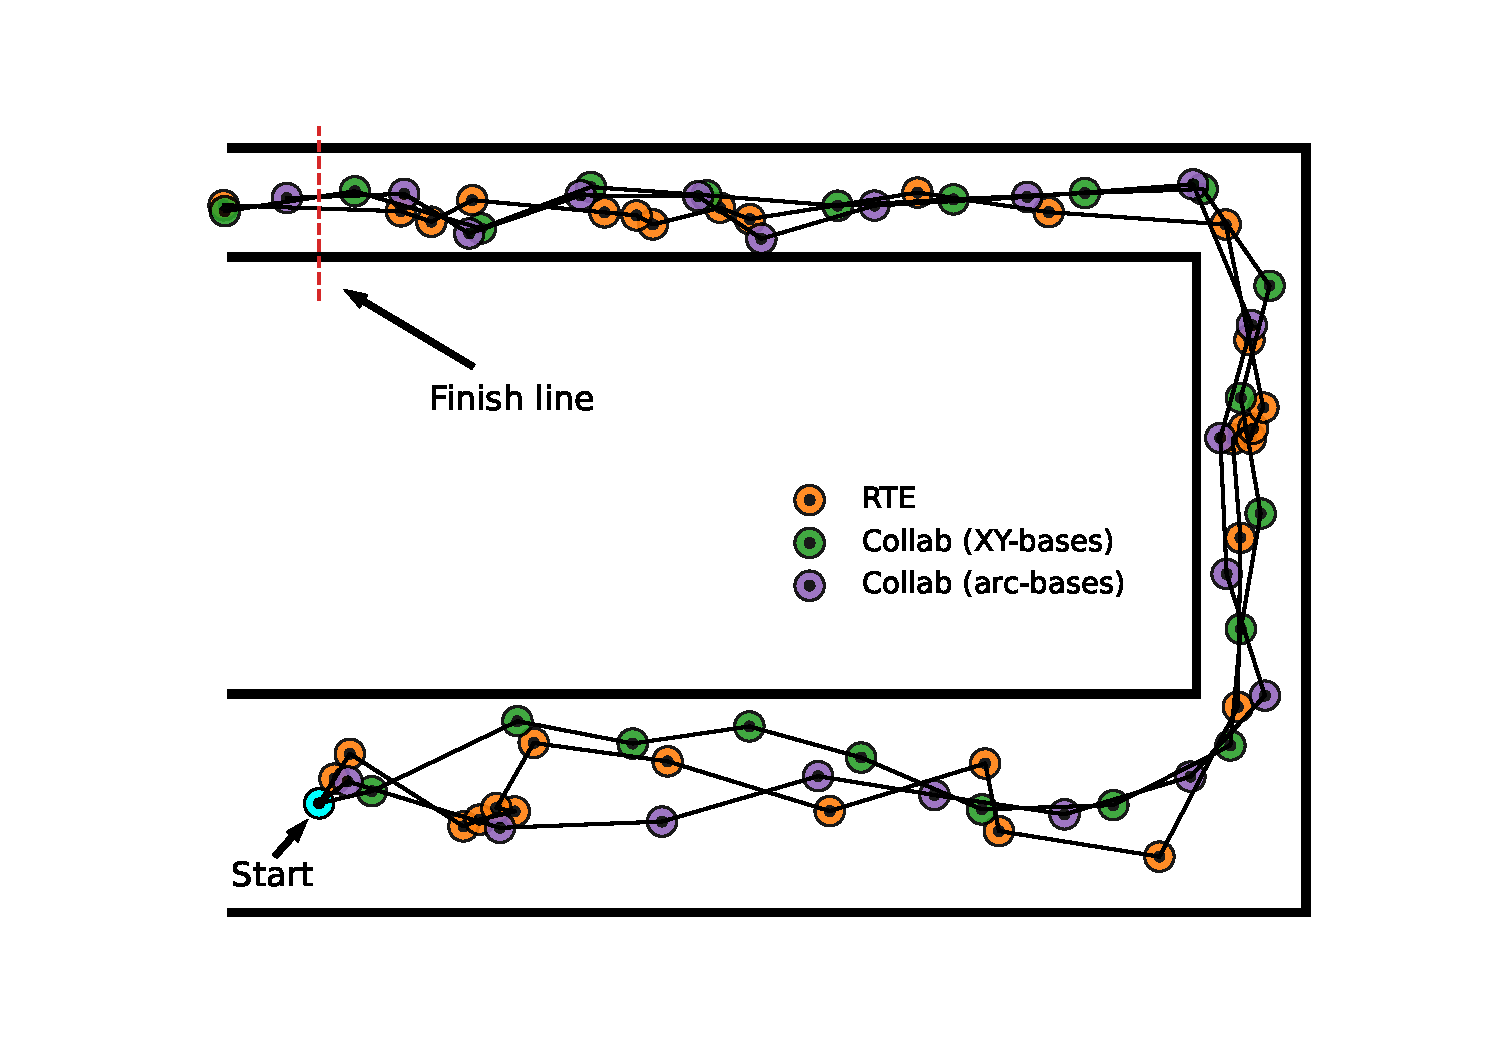
\includegraphics[width=0.45\textwidth]{trajectories.pdf}
\caption{The adaptation progress of the robots in the maze.
The robots are initialized at the center of the starting area facing due right ($0^{\circ}$).
The semitransparent notes connected by dash lines stands for executions that led to collisions.
}
\label{navigation_process}
\end{figure}

It is strange that the arc-based method led to the most collisions in this environment, while RTE has much higher errors in its predictions.
A highly probably explanation is that since the polices are QD-optimized in the default simulation environment, the robot typically moves slower in a different environment.
Since the RTE uses the baseline dynamics as the prior, it overestimates the mobility of the polices.
Hence in many cases, the robot using RTE would select a policy that makes a small step but is also lesser likely to cause collisions.
Our method on the other hand, better predicts the mobility, and a large fraction of the prediction error is on the sideways.
This makes our method always choose a fast moving policy, but the risk of having collisions is higher if the model is not accurate enough.
To validate our analysis, we recorded the adaptation process of the three robots in env 2 (see Fig \ref{navigation_process}).
We can see that there are many steps where the robot using RTE barely moves.  
But with this particular initial state, it made the least number of collisions.
The other two robots both travel very fast with much larger steps.
However, we see more collisions made by these robots especially for the one using arc-based method when passing through the final corridor.
This because the arc-based model has sideways errors too large for this section of the maze, which is consistent with our analysis.
Remember that for simplicity, we did not incorporate the uncertainties of the model predictions into our objective function but gave an universal safe distance of $0.5$ instead.
If we consider the uncertainties for each prediction, the methods would potentially have lesser collisions.